\documentclass{article}
\usepackage[margin=1in]{geometry}
\usepackage{amsmath,amsthm,amssymb,amsfonts, fancyhdr, color, comment, cancel, graphicx, environ}
\usepackage{xcolor, soul}
\usepackage{mdframed}
\usepackage{array}
\usepackage[shortlabels]{enumitem}
\usepackage{indentfirst}
\usepackage{hyperref}
\usepackage{tikz}
\usetikzlibrary{shapes.geometric}
\usepackage{listings}
\usepackage{booktabs}
\hypersetup{
    colorlinks=true
    linkcolor=blue
    filecolor=magenta
    urlcolor=blue
}

\definecolor{customgray}{rgb}{0.90, 0.90, 0.90}
\lstdefinestyle{mystyle}{
    backgroundcolor=\color{customgray},
    basicstyle=\ttfamily\footnotesize,
    breakatwhitespace=false,
    breaklines=true,
    captionpos=b,
    keepspaces=true,
    showspaces=false,
    showstringspaces=false,
    showtabs=false
    tabsize=2
}

\pagestyle{fancy}

\setlength\parindent{0pt}

\lhead{YIP, ZHAO, AND ZHOU}
\chead{PROJECT PROPOSAL}
\rhead{CPSC 437}

\renewcommand{\baselinestretch}{1.25}
\lstset{style=mystyle}

\begin{document}
\sethlcolor{teal}
\section*{Group Members}
Kelvin Yip (netID: khy6), Amy Zhao (netID: axz4), Lily Zhou (netID: yz878) 

\section*{Project Proposal}
\subsection*{Introduction and Data Sources}
We propose a course recommendation system for courses offered at Yale. For any or several selected courses, we will use natural language processing (NLP) to offer a list of related courses that may appeal to the user. We will further sort this list by popularity (i.e. by enrollment numbers). We plan to scrape course data from Yale Course Search (first source) and enrollment statistics from Yale Course Demand Statistics (second source). For a stretch goal, we can consider scraping course data from another Ivy League (e.g. Harvard) to act as a source of comparison to Yale's courses. 

\subsection*{High-Level Implementation}
For our project, we will scrape data from two main data sources: Yale Course Search and Yale Course Demand Statistics. Yale Course Search provides information on courses held at Yale, including course code, course title, course description, course meeting time, and professor. These details will become the attributes of one table in our database. The second table in our database will hold data on enrollment statistics taken from Yale Course Demand Statistics. \\[2mm]
Our proposed database schema can be modeled by the E-R diagram below: 
\begin{center}
    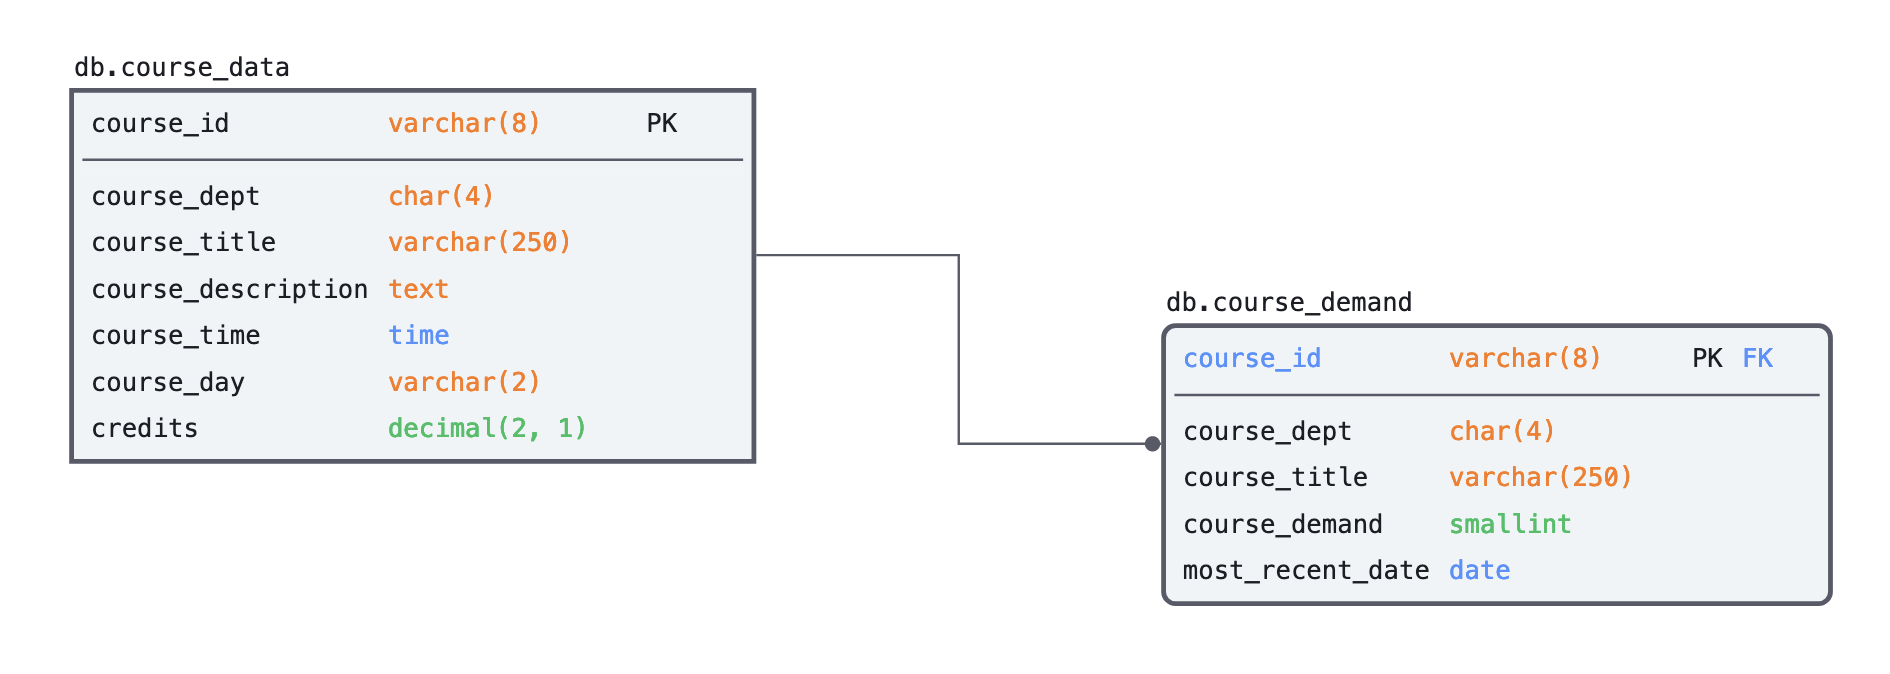
\includegraphics[scale=0.30]{db_schema.png}
\end{center}
Yale Course Search and Yale Demand Statistics are well-defined and most, if not all, courses have all specified database attributes available. \\[2mm]
Note that there is a need to format the data for the purposes of NLP. This will include the removal of stop words, the removal of non-alphanumeric characters, and lemmatization, among other procedures. \\[2mm]
Python affords the easiest (and maybe the best documented) tools for NLP. Many of these tools are found in the Natural Language Toolkit (\texttt{NLTK}) or in \texttt{scikit-learn}. Our course recommendation system will rely on text similarity between the course descriptions of different courses, where the similarity will be determined by cosine similarity. If there are better metrics to measure text similarity, we may also consider using those. \\[2mm]
Using the measure of similarity, we will produce the top five most similar courses to a single selected course. For these top five courses, we will query the course demand database and retrieve the enrollment numbers. We may also implement functionality that allows for a user to select multiple courses and receive a single list of recommendations from that list of selected courses.
 
\end{document}